\documentclass[UTF8, a4paper, linespread=1.5]{article}

\usepackage{tcolorbox, listings, algorithm, minted, algpseudocode}
\usepackage{geometry, savesym, amsmath, enumerate, indentfirst, color, amsthm, bm, extarrows, ulem}
\usepackage{amssymb}
\usepackage{nameref, hyperref}
 \geometry{top=3cm, bottom=3cm, left=1.5cm, right=1.5cm}

\usepackage{enumitem}
\setenumerate[1]{itemsep=0pt,partopsep=0pt,parsep=\parskip,topsep=5pt}
\setitemize[1]{itemsep=0pt,partopsep=0pt,parsep=\parskip,topsep=5pt}

\renewcommand\contentsname{Contents}

\tcbuselibrary{skins, breakable, theorems}

% \setlength{\leftskip}{10pt}
\setlength{\parindent}{10pt}
% \setlength{\parskip}{2em}
\renewcommand{\baselinestretch}{1.3}

\newcounter{RomanNumber}
\newcommand{\mrm}[1]{(\setcounter{RomanNumber}{#1}\Roman{RomanNumber})}

\newtcbtheorem{thm}{}
  {enhanced, theorem name and number, code={\edef\@currentlabelname{#2}}, 
  frame code={
        % \path[thick, draw] (frame.north west) -| (frame.north east) -| (frame.south east) -| (frame.south west) -| (frame.north west);
        \path[thick, draw] (frame.north west)  +(.5\baselineskip,0) -| +(0,-.5\baselineskip);
        % \path[thick, draw] (frame.north east) +(-.5\baselineskip,0) -| +(0,-.5\baselineskip);
        % \path[thick, draw] (frame.south west) +(.5\baselineskip,0) -| +(0,.5\baselineskip);
        \path[thick, draw] (frame.south east) +(-.5\baselineskip,0) -| +(0,.5\baselineskip);
    },
    left=1mm, right=1mm, top=1mm, bottom=1mm,
    colback=black!5,
    colframe=red!75!black,
    colbacktitle=black!0,
    coltitle=black!100,
    fonttitle=\bfseries}{thm}


\usepackage{environ}
\RenewEnviron{math}{%
\begin{align*}
\BODY
\end{align*}
}

\title{CS217 -- Algorithm Design and Analysis \\ Homework 5}
\date{\today}
\author{Not Strong Enough}



\begin{document}
    \maketitle

    \begin{thm}{}{}
        Let $T$ be a minimum spanning tree of $G$, and let $c\in \mathbb{R}$.
        Show that $T_c$ and $G_c$ have exactly the same connected components. (That is, two vertices $u,v\in V$ are connected in $T_c$ if and only if they are connected in $G_c$).
        You are encouraged to draw pictures to illustrate your proof.
    \end{thm}
    \begin{proof}[Solution]
        Since $T_c$ is a subgraph of $G_c$, if $u,v\in V$ are connected in $T_c$, then $u,v$ are connected in $G_c$.
        
        Now let's assume $u,v\in V$ are not connected in $T_c$, but are connected in $G_c$.
        Then, the path in $T$ from $u$ to $v$ contains an edge $y$ whose weight is greater than c.
        Also, there exists a path $P$ in $G$ from u to v such that $\forall e\in P, w(e)\leq c$.
        If we remove $y$ from $T$, $T$ will be split into 2 connected components where u belongs to one and v belongs to another.
        So there must be an edge $x\in P$ whose endpoints belongs to different connected components.
        Adding $x$ into $T$ then will make the 2 components connected again.
        Let $T'=T+x-y$.
        Now $T'$ becomes a tree, because it has $|V|-1$ edges and it's connected.
        The total weight of  $T'$ is $w(T)+w(x)-w(y)<w(T)$, which violates that $T$ is an MST\@.
        So $u,v$ are not connected in $G_c$ if they are not connected in $T_c$.

        In conclusion, two vertices $u,v\in V$ are connected in $T_c$ if and only if they are connected in $G_c$.
    \end{proof}

    \newpage
    
    \begin{thm}{}{}
        For a weighted graph $G$, let $m_c(G) := | \{e \in E(G) \mid w(e) \leq c\}|$, i.e., the number of edges of weight at most $c$ (so $G_c$ has $m_c(G)$ edges). Let $T$, $T'$ be two minimum spanning trees of G. Show that $m_c(T) = m_c(T')$.
    \end{thm}
    
    \begin{proof}
        For a graph $G = (V, E)$, from the definition of $m_c(G)$ we have $m_c(G) = | \{e \in E(G) \mid w(e) \leq c\} | = |E(G_c)|$. Since $T$ and $T'$ are two minimum spanning trees of $G$, by the conclusion of exersice 1, we know that $T_c$ and $G_c$ have exactly the same connected components, and $T'_c$ and $G_c$ also have the same connected components. It follows that $T_c$ and $T'_c$ have the same connected components.
        
        Note that $T_c$ and $T'_c$ are two \textit{forests}. We know that for a forest with $n$ nodes and $k$ connected components, there are exactly $n - k$ edges in the forest. Hence $T_c$ and $T'_c$ having the same connected components means that the number of edges in $T_c$ and $T'_c$ are also the same, i.e., $m_c(T) = m_c(T')$.
    \end{proof}

    \newpage
    
    \begin{thm}{}{}
        Suppose G is connected, and no two edges of G have the same weight. Show that G has exactly one minimum spanning tree.
    \end{thm}

    \begin{proof}[Proof]
        Suppose there are two different minimum spanning trees, named $T$ and $T'$. 
        
        Now we remove an edge $e$ in $T$, and the graph becomes two connected parts. 
        If in $T'$ the two parts are connected by $e$ too, 
        then remove another edge in $T$ until the one in $T'$ is different from the one in $T$, 
        and we name the one in $T'$ be $e'$ in this case. 
        
        There should be such a pair $(e,e')$: 
        otherwise, each edge in $T$ is the same as that in $T'$, which is a contradiction. 
        
        Now consider such pair$(e,e')$. Without loss of generality, assume that $w(e)<w(e')$. 
        Then if we replace $e'$ in $T'$ by $e$, the total weight of $T'$ is less, so $T'$ is not a minimum spanning tree. 
    \end{proof}

    \newpage
    
    A \textit{multigraph} is a graph that can have multiple edges, called ``parallel edges''. Without defining it formally, we illustrate it:
    \begin{center}
        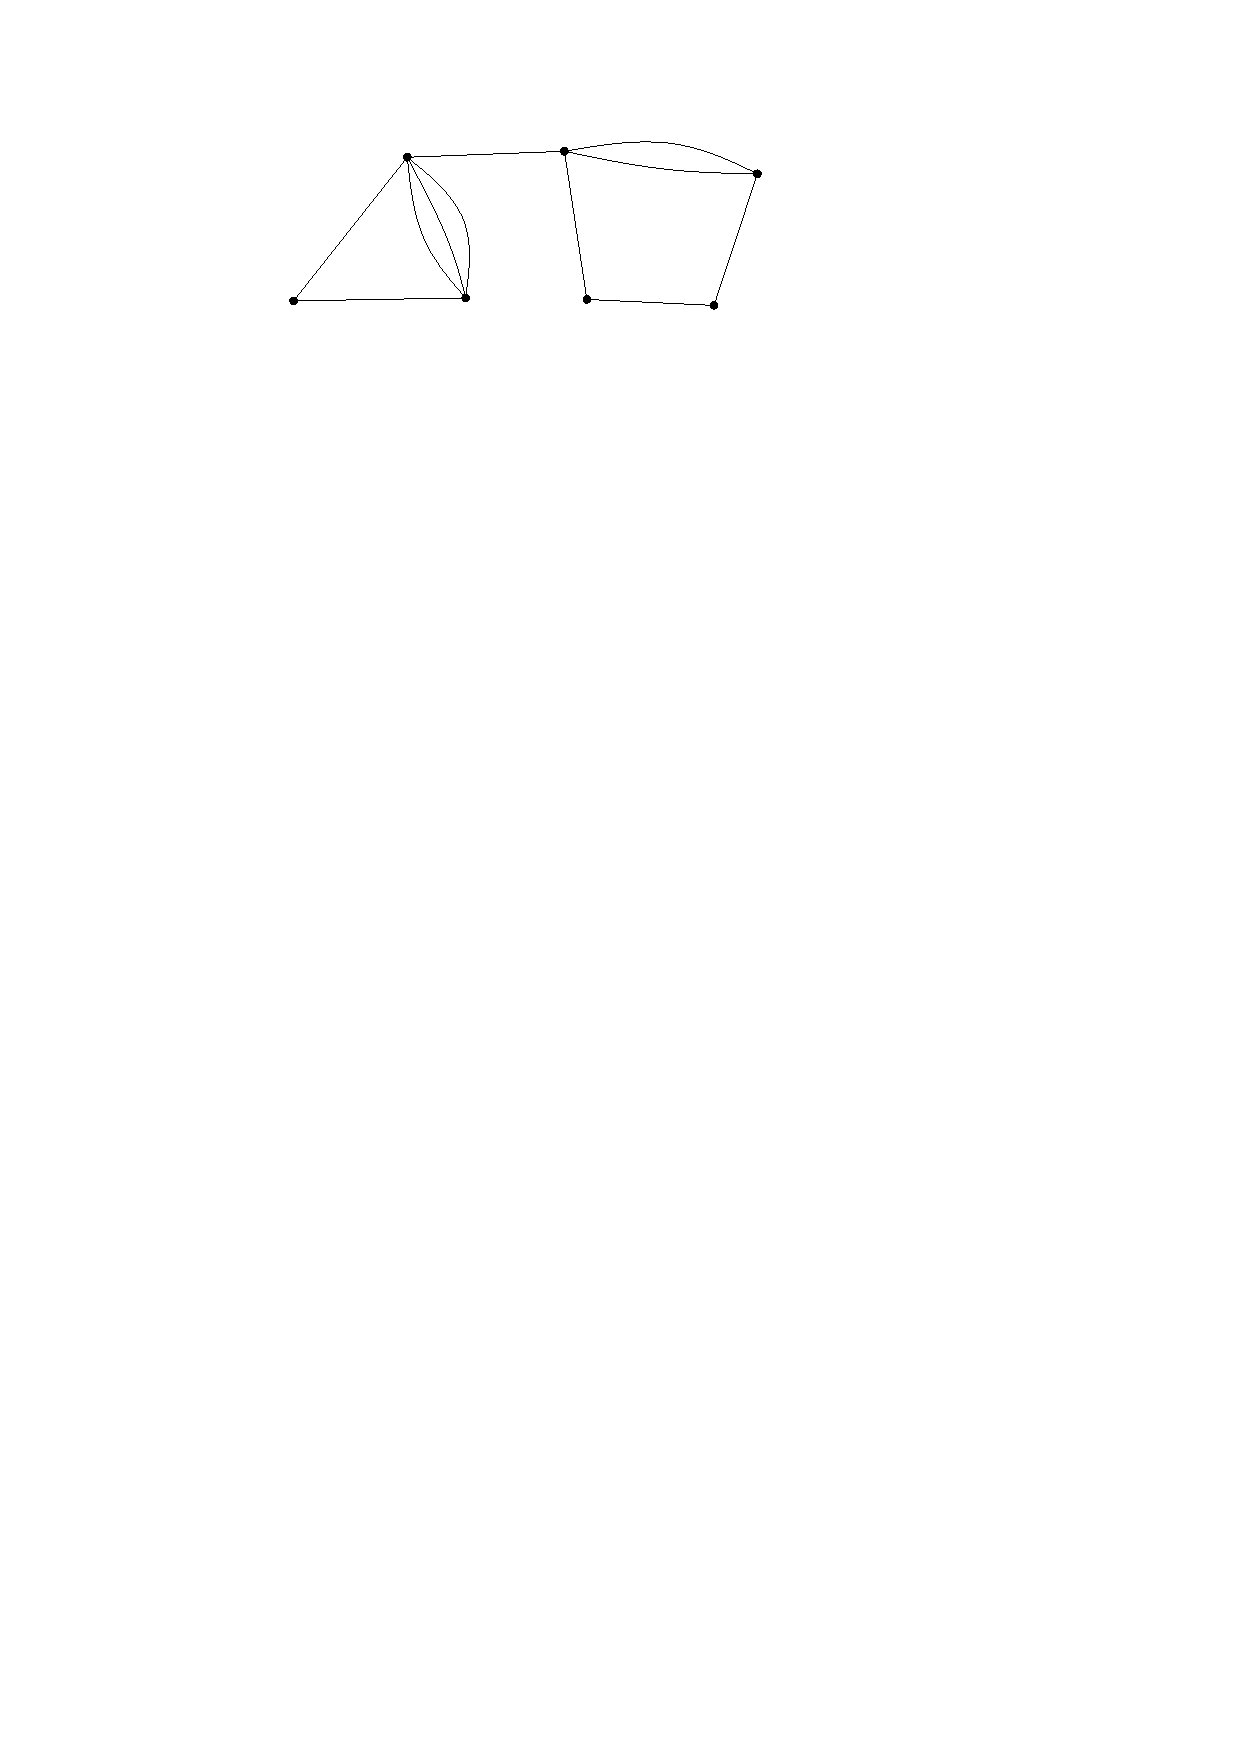
\includegraphics[width=0.4\textwidth]{T4/figures/multigraph.pdf}\\
        A multigraph.
    \end{center}
    All other definitions, like connected components and spanning trees are the same as for normal (simple) graphs. However, when two spanning trees use different parallel edges, we consider them different:
    \begin{center}
        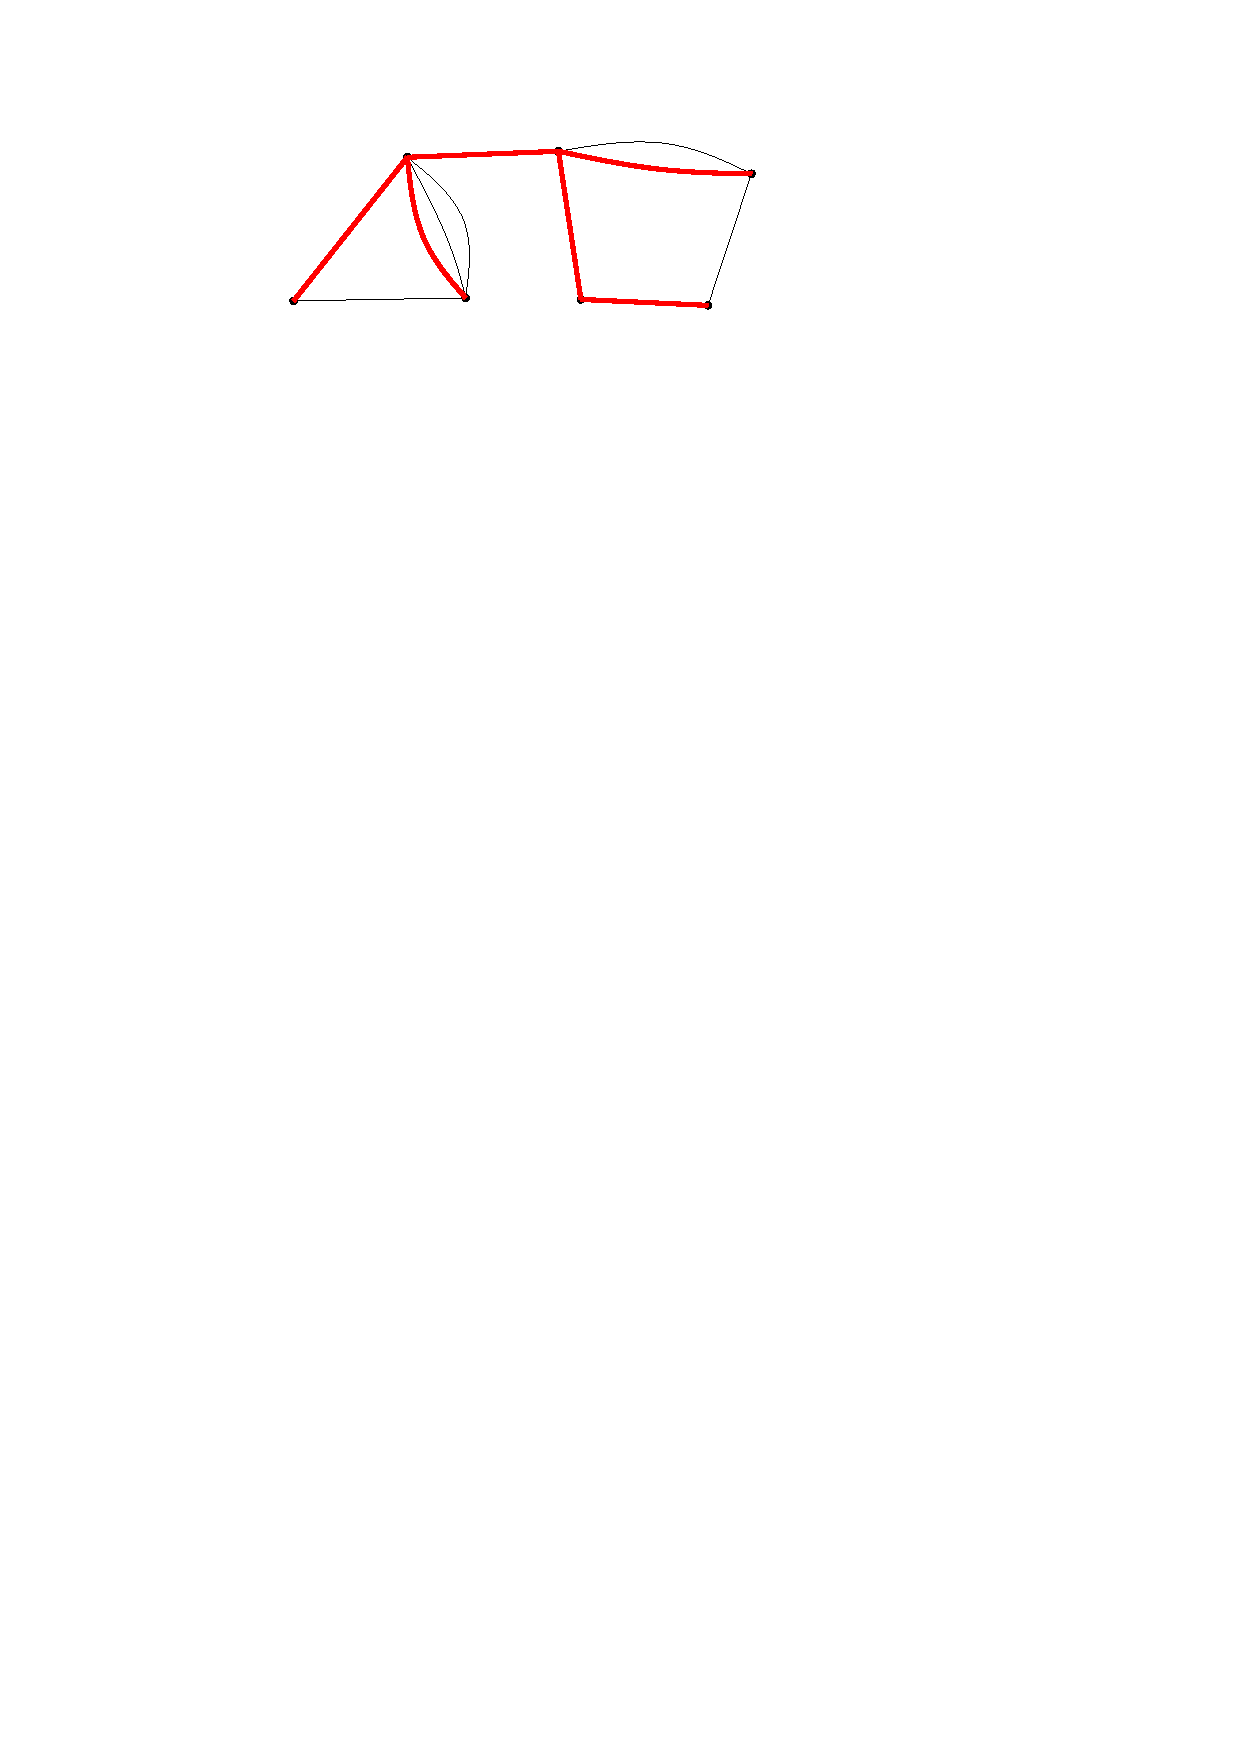
\includegraphics[width=0.3\textwidth]{T4/figures/multigraph-forest.pdf} \hspace{2cm}
        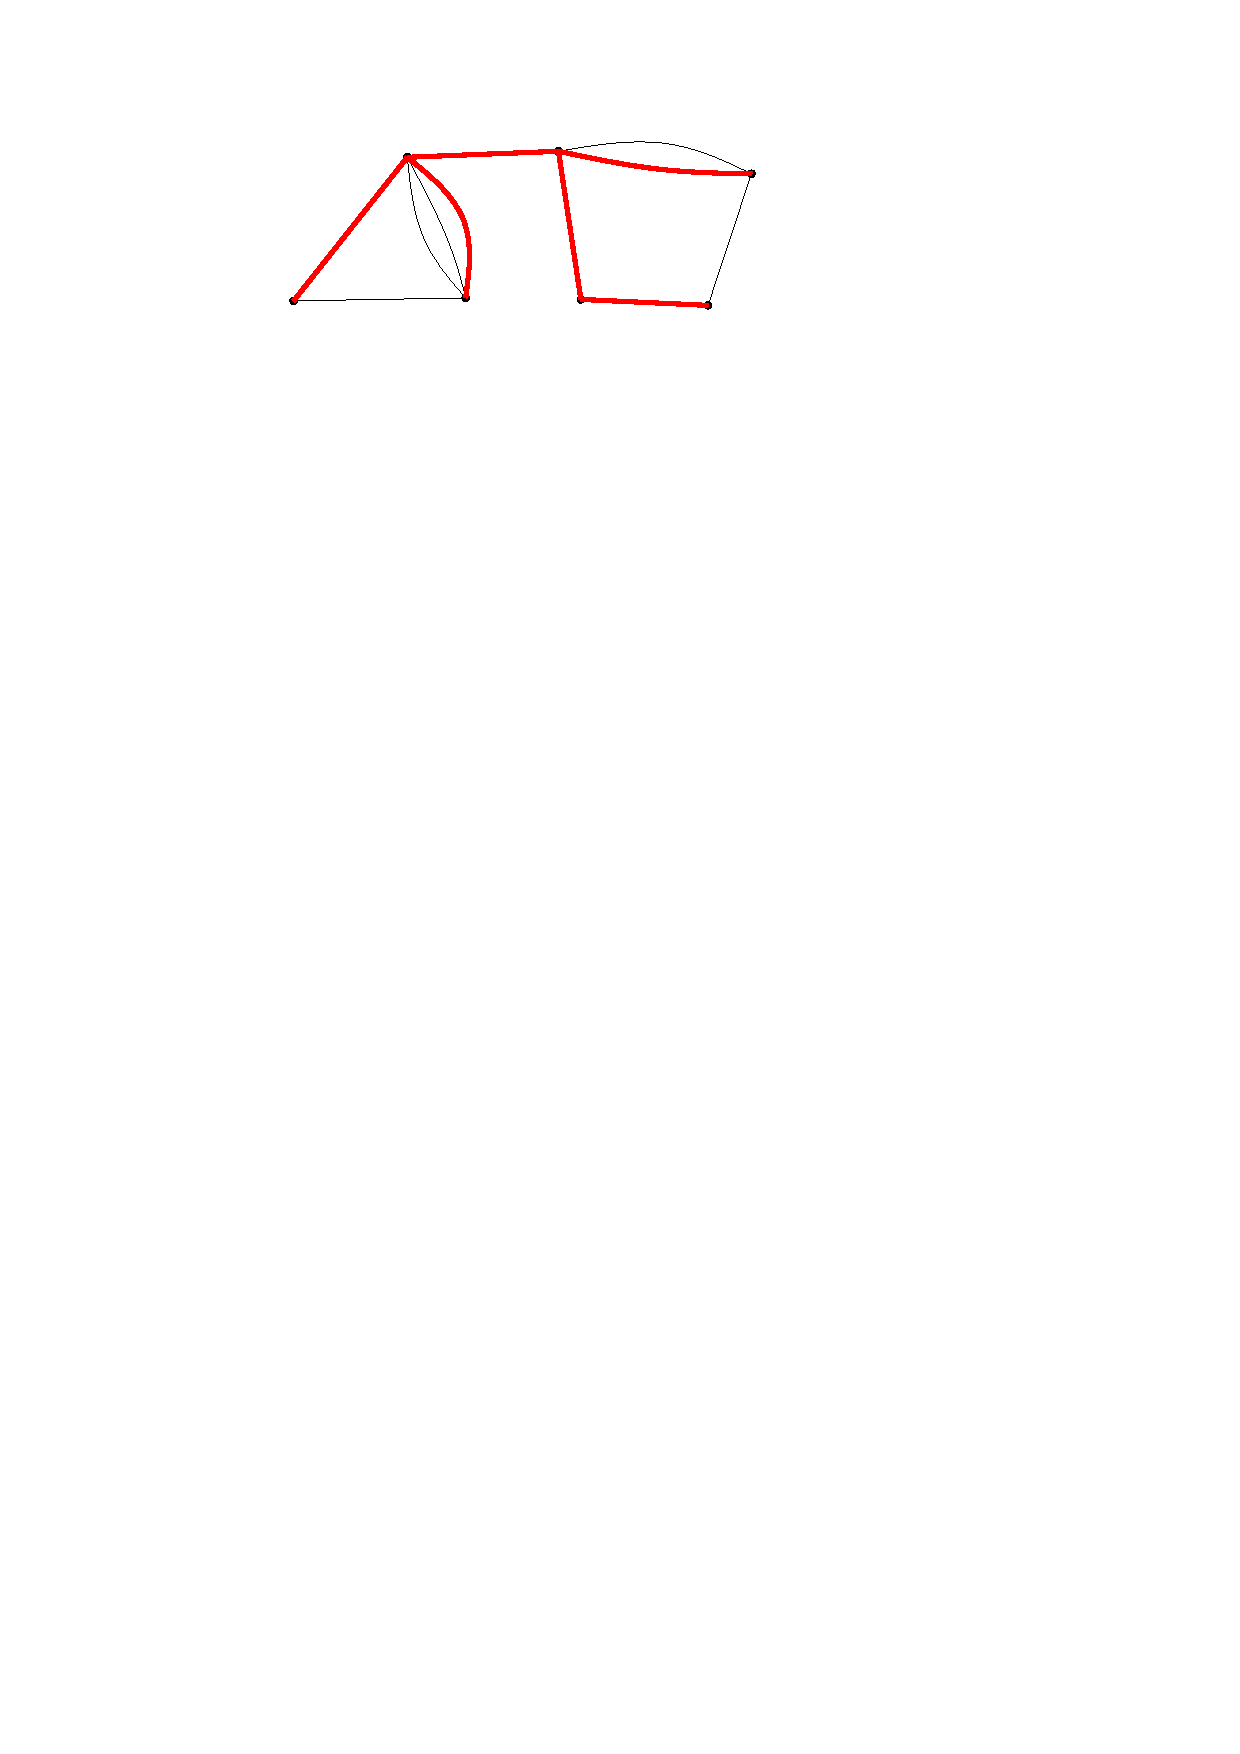
\includegraphics[width=0.3\textwidth]{T4/figures/multigraph-forest-other.pdf} \\
        The same multigraph with two different spanning trees.
    \end{center}
    
    \begin{thm}{}{}
        How many spanning trees does the above multigraph on 7 vertices have? Justify your answer!
    \end{thm}
    
    \begin{proof}[Solution]
        Firstly, we label the 7 vertices from $a$ to $g$ as below.
        \begin{center}
            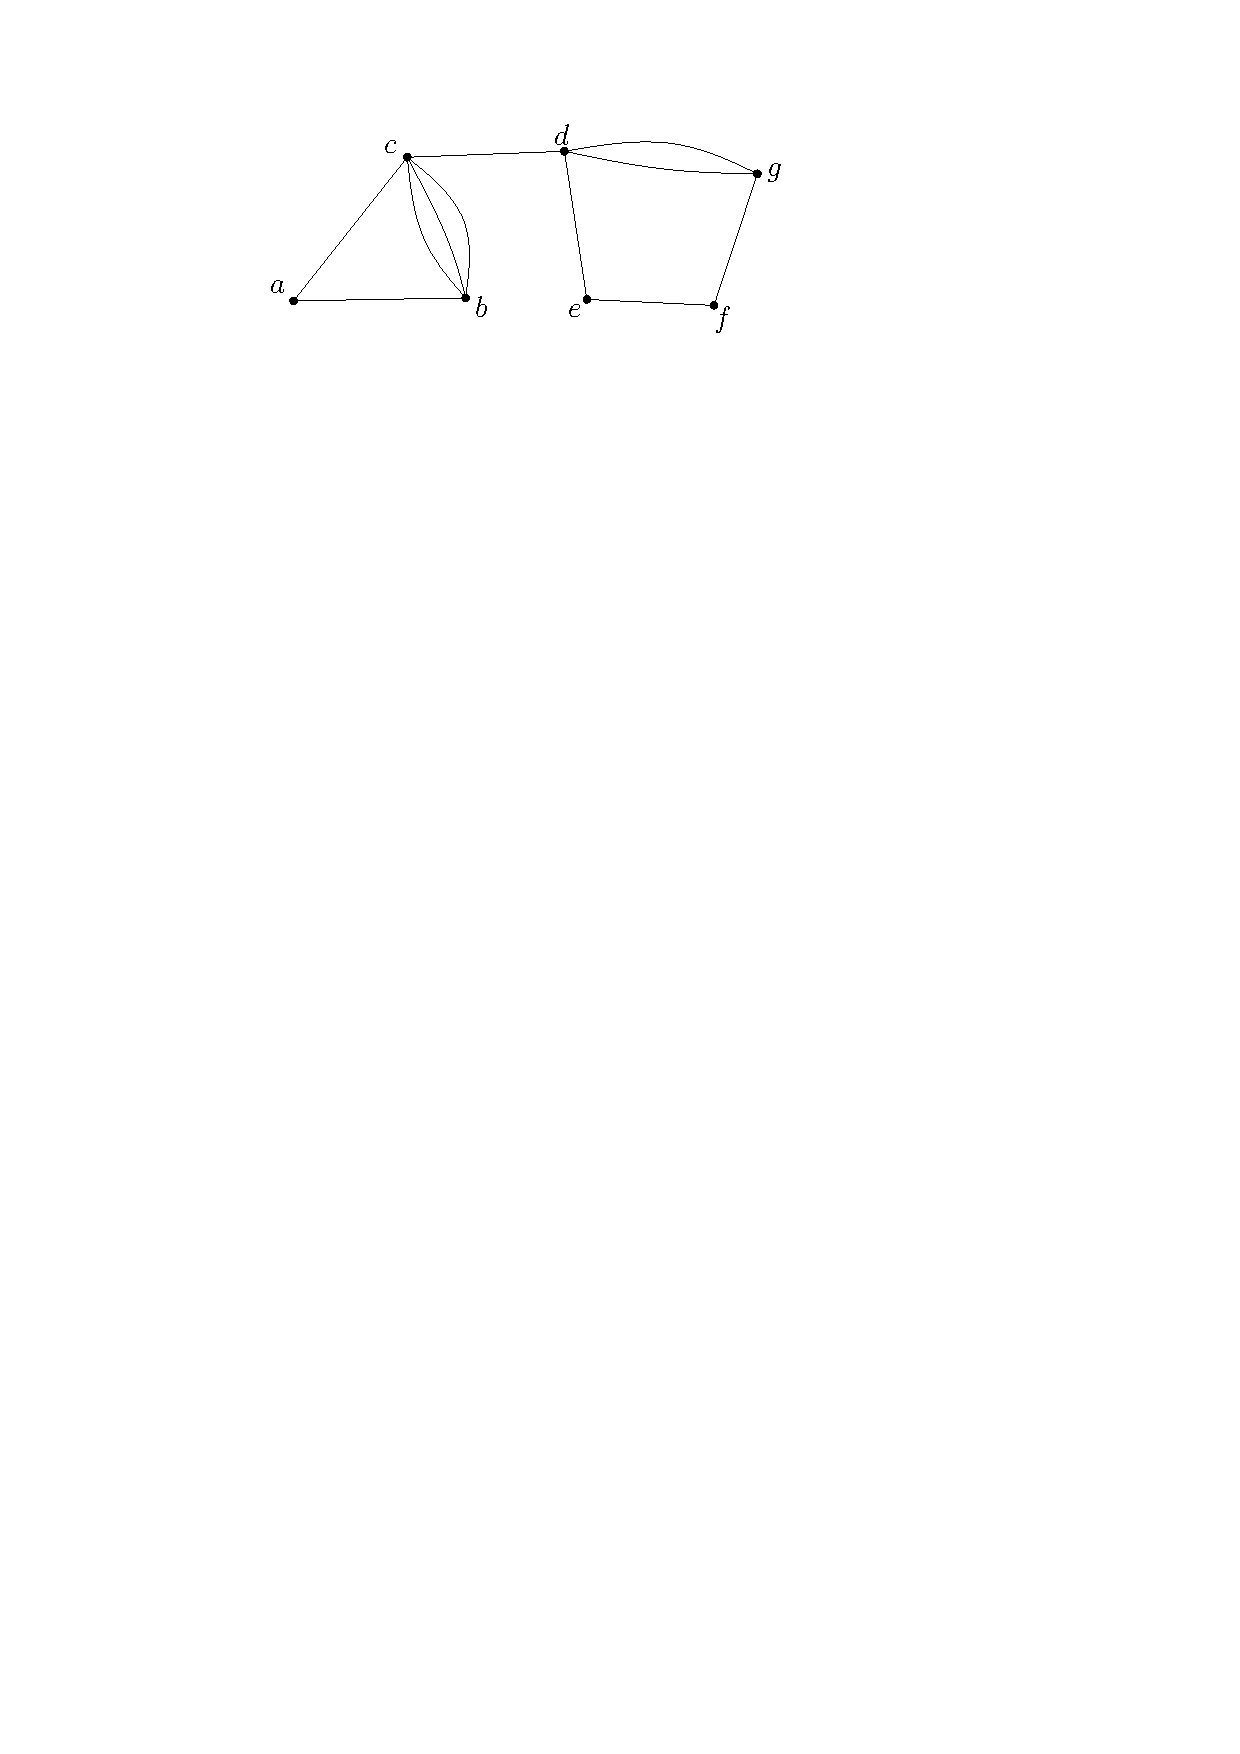
\includegraphics[width=0.4\textwidth]{T4/figures/multigraph-labeled.pdf}
        \end{center}
        
        Obviously, as a bridge, the edge $\{c, d\}$ is contained in every spanning tree. So we only need to count the number of spanning trees of vertices $V_1 = \{a, b, c\}$ and $V_2 = \{d, e , f, g\}$ respectively, and then multiplying the two numbers we get the number of spanning trees of the original graph.
        \begin{center}
            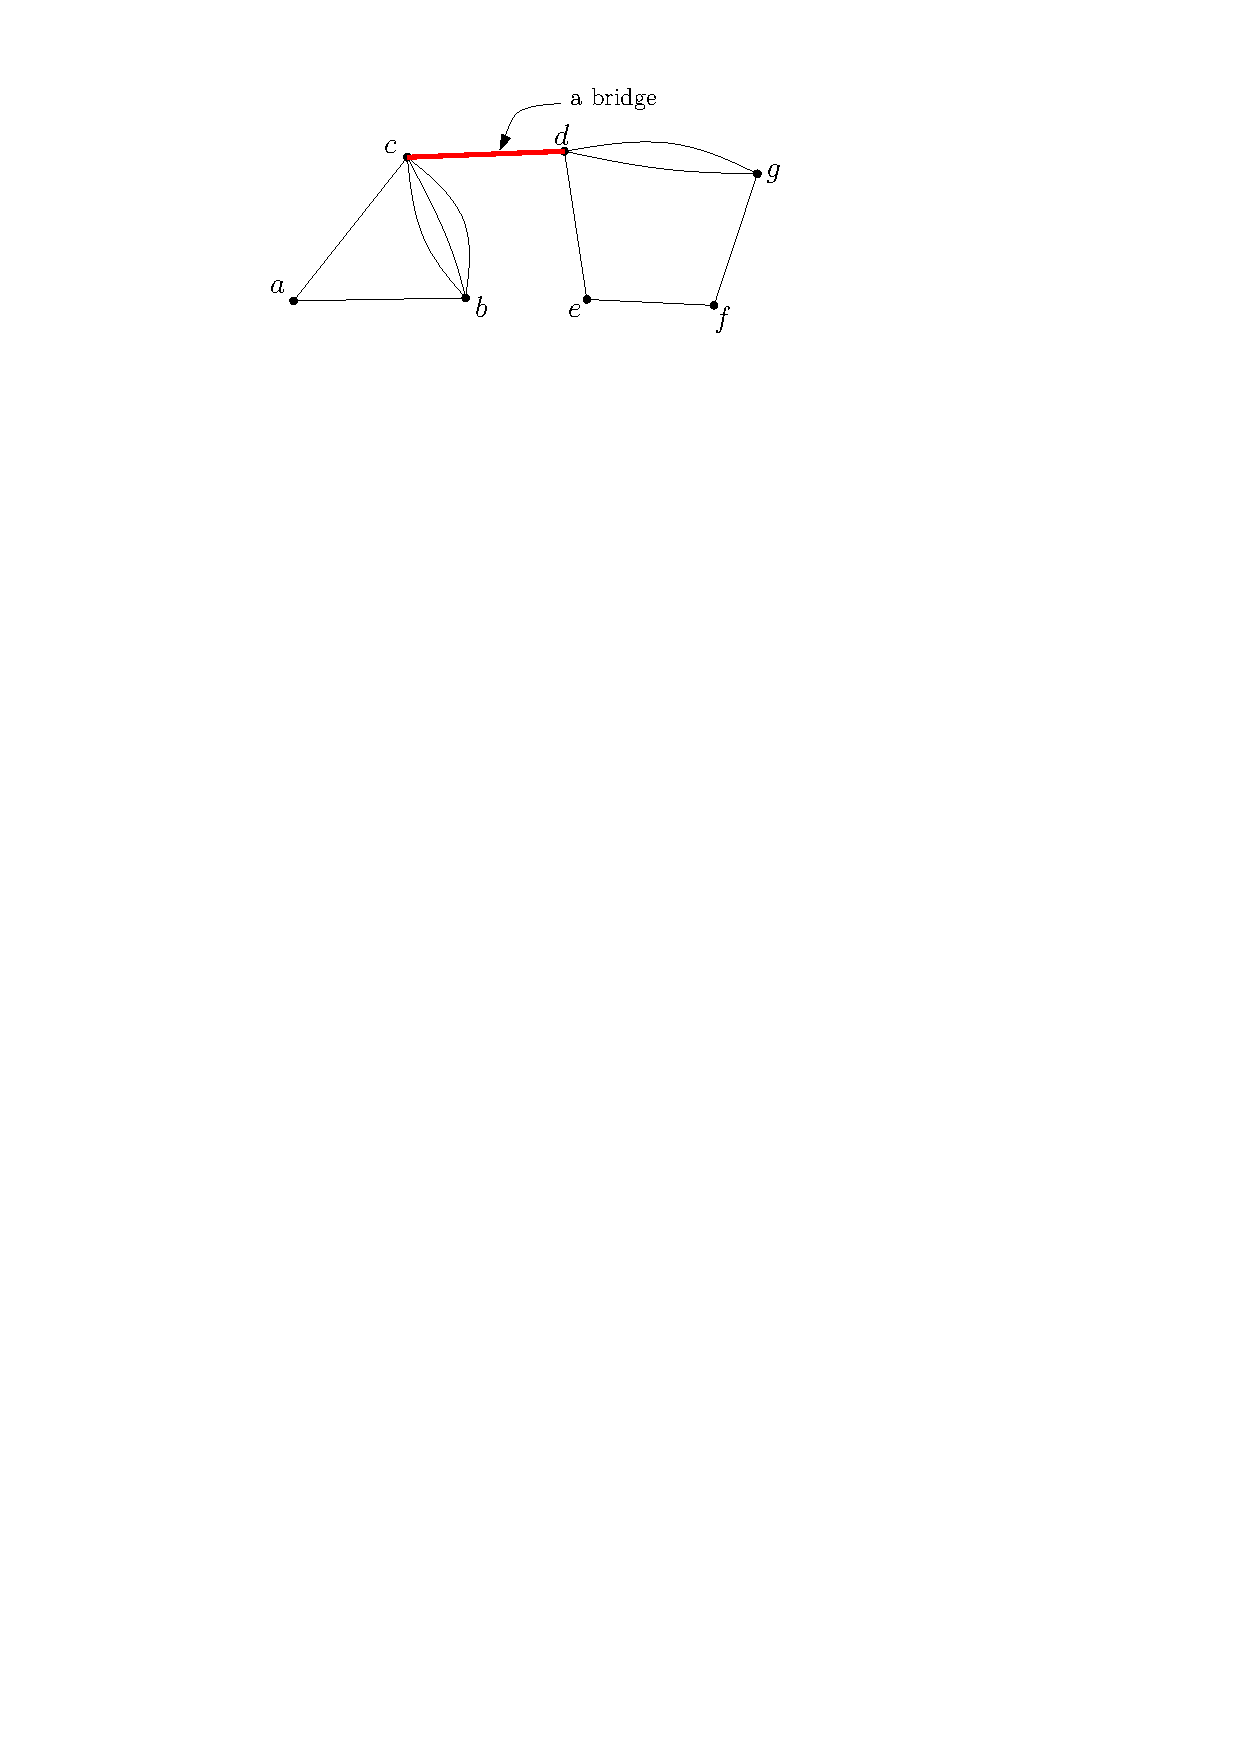
\includegraphics[width=0.4\textwidth]{T4/figures/multigraph-bridge.pdf}
        \end{center}
        
        Consider the sub-multigraph with vertices $a$, $b$ and $c$. If we select none of the edges between $b$ and $c$, there are only $1$ spanning tree. Otherwise we select one of the edges between $b$ and $c$, and we can select another edge which is either $\{a, c\}$ or $\{a, b\}$. So there are $cnt_l = 1 + 2 \times 3 = 7$ spanning trees in the left sub-multigraph.
        
        Then we consider the right sub-multigraph with vertices $d$ to $g$. Similarly, there is only one spanning tree which doesn't contain an edge between $d$ and $g$. And if we select an edge between $d$ and $g$, the other two edges can be any two among $\{d, e\}$, $\{e, f\}$ and $\{f, g\}$. So there are $cnt_r = 1 + 3 \times 2 = 7$ spanning trees in the right sub-multigraph.
        
        Finally we multiply $cnt_l$ and $cnt_r$. So the total number of spanning trees in the given multigraph is $cnt_l \times cnt_r = 7 \times 7 = 49$.
    \end{proof}
    
    \newpage
    
    \begin{thm}{}{}
        Suppose you have a polynomial-time algorithm that, given a multigraph $H$, computes the number of spanning trees of $H$. Using this algorithm as a subroutine, design a polynomial-time algorithm that, given a weighted graph $G$, computes the number of minimum spanning trees of $G$.
    \end{thm}
    
    \begin{algorithm}
        \caption{Compute the number of minimun spanning tree of $G$}
        \begin{algorithmic}
            \Function{NumberOfSpanningTreesOfMultigraph}{$V$, $E$}
            
            some black magic...
            
            \EndFunction
            
            \Function{NumberOfMST}{$V$, $E$, $w$}
            
            \State $W \gets [w(e_i): e_i \in E]$
            \State sort $W$ so that $i < j \iff w_i < w_j$
            \State $X \gets \varnothing$
            \State $Answer \gets 1$
            
            \For{$w_i \in W$}
            
            \State $E_{w_i} \gets \{e_i: w(e_i) = w_i\} $
            \State $V' \gets$ connected components of $G' = (V, X)$
            \State $E' \gets \{(A, B): (x, y) \in E, x \text{ is in component } A, y \text{ is in component } B\}$
            \State $Answer \gets Answer \times$ \Call{NumberOfSpanningTreesOfMultigraph}{$V'$, $E'$}
            \State $X \gets X \cup E_{w_i}$
            
            \EndFor
            
            \Return $Answer$
            
            \EndFunction
        \end{algorithmic}
        
    \end{algorithm}
    
    The algorithm above can compute the number of MST of $G$ in polynomial time if we can get the number of spanning trees of multigraphs in polynomial time.
    \begin{itemize}
        \item Effectiveness(polynomial-time):
        
        It is polynomial-time because the for-loop will be executed $O(|E|)$ times, and every statement in the loop can be done in polynomial time.
        
        \item Correctness:
        
        Consider the process of Kruskal's Algorithm to find an MST, [problem 1] shows that $T_{w_i}$ will always have the same connected components. Thus, by adding edges of same weights into that graph, the resulting connected components will always be the same. This observation indicates that there will be multiple MSTs if and only if we can add $E_{w_i}$ into the graph in different ways, and for every $w_i$, the influence on answer is independent.
        
        Thus at each time we add edges of same weights into the graph together, and find the number of ways these edges can connect the current graph. The number of MSTs is the product of numbers of ways for every $w_i$.
        
        
    \end{itemize}
\end{document}

